% Art der Arbeit: Bachelorarbeit
% Titel: "BLAST Avionics Thermal Management"
% Autor: Viktor Hoffmann
%-----------------------------------------------------------------------------------
% verwendete Packages
\documentclass{ITLR}
% Use ITLR.cls for first style-definition. 
% IMPORTANT: change in ITLR.cls colors in hyperref-package ONLY for printing; NOT for PDF submittance


% ----------- Zusätzliche Usepackages ----------------------------------------------
% Hier stehen weitere Usepackages ...
\usepackage{siunitx}
\usepackage{tikz}
\usepackage{subcaption}
\usetikzlibrary{arrows.meta}
\usepackage{acronym}

% ----------- Graphics Paths -------------------------------------------------------
\graphicspath{{Bilder/}}

%###################################################################################
% ----------- Dokumentanfang -------------------------------------------------------
\begin{document}
\setstretch{1.1667} 		% Zeilenabstand (Verhältnis, hier z.B. 14pt/12pt)
\pagestyle{Abstract}		% oben definiert

% ----------- Title & Preface  -----------------------------------------------------
\pagenumbering{Alph}
\begin{titlepage}
%---- ITLR-Logo ----
\begin{figure}[ht]
     \centering
      \includegraphics[width=65mm]{./Logos/ITLR_Logo.eps}
\end{figure}

\hspace{200mm}

%---- Title of the study thesis ----
\begin{center}
    \begin{Large}
        Bachelorarbeit
    \end{Large}

    \vspace{2.5mm}

    \BRule
    \vspace{2.5mm}
    \begin{LARGE}
    \\
        Entwicklung des Avionik-Thermal-Managements einer Experimentalrakete
        \\
    \vspace{1mm}
    \end{LARGE}
    \vspace{2.5mm}
    \BRule
    \vspace{15mm}

    \begin{Large}

    Viktor Hoffmann \\
    
\end{Large}

\end{center}

\vfill

%---- Uni-Logo ----
\begin{wrapfigure}[4]{l}{17mm}
    
\includegraphics[width=17mm]{./Logos/unilogo_neu}
\end{wrapfigure}

\parbox[t]{120mm}
{
    \sffamily
      \vspace{3mm}
        Universität~Stuttgart\\
        \textbf{Institut~für~Thermodynamik~der~Luft-~und~Raumfahrt~(ITLR)}\\[2mm]
        Direktor: Prof.~Dr.-Ing.~habil.~Bernhard~Weigand
}




\end{titlepage}


% erste Seite: Titelblatt (wird von ITLR erstellt)
% zweite Seite: leeres Blatt
% dritte Seite: Aufgabenstellung (wird von ITLR erstellt)
% vierte Seite: Erklärung (wird von ITLR erstellt, muss aber noch unterschrieben werden)

\pagenumbering{Roman}		% Am Anfang römische Seitenzahlen
% ----------- Abstract -------------------------------------------------------------
\newpage
\phantomsection		% Korrigiert die Hyperref-Verlinkungen
\addcontentsline{toc}{chapter}{Kurzzusammenfassung} %\addcontentsline
\chapter*{Kurzzusammenfassung} % * means not in table of content
\label{chap:Kurzzusammenfassung}

% ca. 150 Worte / Aufgabenstellung, Zielsetzung, verwendete Methoden, Ergebnisse kurz vorstellen, aber nicht diskutieren / Leser entscheidet hier, ob er die Arbeit für lesenswert hält

% deutsch
Für das Projekt \ac{blast} der Hochschulgruppe \ac{hyend} wird eine neue, kompakte und hochleistungsfähige Avionik entwickelt,
die unter extremen Flugbedingungen arbeitet. Die in dieser Arbeit entwickelte Kühlung muss leicht, ausfallsicher und für eine
maximale Sperrschichttemperatur von $T_\mathrm{J} \approx T_\mathrm{C} \leq \SI{85}{\celsius}$ für die gesamte Missionsdauer ausgelegt sein.
Basierend auf den Anforderungen und einer Trajektoriensimulation
wurden drei Konzepte untersucht: reiner Radiator, reines \ac{pcm} und eine hybride Radiator-\ac{pcm}-Lösung. Die Vorauslegung
ergab, dass ein Radiator wegen aerothermaler Aufheizung ungeeignet ist. Die hybride Lösung ist möglich, jedoch durch geometrische
Verluste und hohe Luftwärmeströme der Vorauslegung nach mit \SI{3.835}{\kilogram} schwerer als ein einfaches \ac{pcm}
mit \SI{0.316}{\kilogram}. \ac{cht}-Simulationen der Außenströmung und des \ac{pcm}
bestätigten trotz angenommener Vereinfachungen die Vorauslegungsergebnisse mit einer Masse des hybriden Radiator-\ac{pcm} von \SI{1.522}{\kilogram}.

\chapter*{Abstract} % * means not in table of content
\label{chap:Abstract}
Advanced avionics systems are essential to the success of any experimental rocket.
Ranging from flight computers, telecommunications, and data acquisition to the control
of onboard instrumentation and the rocket itself, high-power microelectronics play a critical role and are often implemented with redundancy.
These systems must be highly compact and capable of withstanding demanding flight conditions, which lead to elevated
power densities that, if not properly managed, can significantly reduce operational lifetime or even cause premature mission failure.
Such is the case in the project \ac{blast} where a novel avionics system is being developed by \ac{hyend} and in need of a thermal management solution.\\

In a first step the demands on the thermal management were set to a maximum junction temperature

% ----------- Verzeichnisse --------------------------------------------------------
% Inhaltsverzeichnis, Abbildungsverzeichnis, Tabellenverzeichnis, Nomenklatur 
\newpage
\tableofcontents	% Erstellt automatisch die Überschrift "Inhaltsverzeichnis" mit

% Tabellenverzeichnis
\newpage
\phantomsection		% Korrigiert die Hyperref-Verlinkungen
\pagestyle{VerzeichnisseNomenklatur}		% wie oben definiert
\addcontentsline{toc}{chapter}{Tabellenverzeichnis} 	% Eintrag ins InhaltsVZ
\listoftables

% Abbildungsverzeichnis
\newpage
\phantomsection		% Korrigiert die Hyperref-Verlinkungen
\addcontentsline{toc}{chapter}{Abbildungsverzeichnis}
\listoffigures				

% Symbolverzeichnis
\newpage
\phantomsection		% Korrigiert die Hyperref-Verlinkungen
\addcontentsline{toc}{chapter}{Symbolverzeichnis}
\chapter*{Symbolverzeichnis}
	
\subsection*{Lateinische Symbole}

\begin{supertabular}{p{10mm}p{3mm}p{20mm}p{3mm}l}
$T$ && \SI{}{\kelvin} && Temperatur\\
$c$ && \SI{}{\joule\per\kilogram\per\kelvin} && Spezifische Wärmekapazität\\
$h$ && \SI{}{\joule\per\kilogram} && Spezifische Schmelzenthalpie\\
\end{supertabular}


\subsection*{Griechische Symbole}

\begin{supertabular}{p{10mm}p{3mm}p{20mm}p{3mm}l}
$\rho$ && \SI{}{\kilogram\per\cubic\meter} && Dichte\\
$\lambda$ && \SI{}{\watt\per\meter\per\kelvin} && Wärmeleitfähigkeit\\
$\gamma$ && \SI{}{\per\kelvin} && Wärmeausdehnungskoeffizient\\
$\epsilon$ && && Emissionsgrad\\
$\alpha$ && && Absorptionsgrad\\
\end{supertabular} 

\subsection*{Indizes}

\begin{supertabular}{p{10mm}p{3mm}p{20mm}p{3mm}l}
solidus && && Solidus Temperatur des Phasenwechsels\\
liquidus && && Liquidus Temperatur des Phasenwechsels\\
solid && && Feststoff Eigenschaften\\
liquid && && Flüssigstoff Eigenschaften\\
fus && && Schmelz Phasenwechsel\\
p && && Konstanter Druck\\
J && && Sperrschicht\\
C && && Gehäuse\\
safety && && Mit Sicherheitsfaktor 1.5\\
t && && spektral integriert\\
s && && solar\\
\end{supertabular} 

\subsection*{Konstanten}

\begin{supertabular}{p{10mm}p{3mm}p{50mm}p{3mm}l}
$\pi$ && $\approx \SI{3.142}{\kelvin}$ && Kreiszahl\\
$\sigma$ && $\approx \SI{3.67e-8}{\watt\per\meter\squared\per\kelvin\tothe{4}}$ && Stefan-Boltzmann-Konstante\\
\end{supertabular}

\newpage

%---Akronyme
\subsection*{Abkürzungen}
\begin{acronym}[BLAST]
\acro{pcm}[PCM]{Phase Change Material}
\acro{pcb}[PCB]{Printed Circuit Board}
\acro{blast}[BLAST]{Biliquid launch and Space Technology}
\acro{fcc}[FCC]{Flight Control Computer}
\acro{hyend}[HyEnD]{Hybrid Engine Development}
\acro{cfd}[CFD]{Computational Fluid Dynamics}
\acro{cht}[CHT]{Conjugate Heat Transfer}
\acro{pgs}[PGS]{Pyrolithic Graphite Sheet}
\acro{maxq}[max~Q]{Maximaler dynamischer Druck}
\acro{gse}[GSE]{Ground Support Equipment}
\acro{pcdu}[PCDU]{Power Control and Delivery Unit}
\acro{atm}[ATM]{Avionik-Thermal-Management}
\acro{rom}[ROM]{Reduced Order Model}
\acro{udf}[UDF]{User Defined Function}
\end{acronym}

% ----------- Verzeichnisse Ende-----------------------------------------------------
\newpage
\pagestyle{main}			% ab hier: normale Kopf- und Fußnoten
% ----------- Einleitung ------------------------------------------------------------
\chapter{Einführung}			
\label{sec:Introduction}
\pagenumbering{arabic}		%ab hier: arabische Seitenzahlen (Hauptteil)

% Problemstellung und Lösungsansätze, 2-3 Seiten / keine Ergebnisse & Folgerungen /

Die Avionik ist ein Grundstein jeder erfolgreichen Experimentalrakete. Ob es hierbei um Telekommunikation,
Datenerfassung oder auch aktive Steuerung und Regelung von
Instrumenten und dem Fahrzeug während des Flugs geht, kompakte Hochleistungsmikroelektronik ist immer gefragt und muss oft redundant ausgeführt sein.
Diese Elektronik, die zudem noch extremen Bedingungen ausgesetzt wird, kommt jedoch mit einer
substanziellen Wärmeleistung und Wärmestromdichte die, bei mangelhafter Rücksicht zu reduzierter Lebensdauer der Avionik führt,
oder sogar die Mission frühzeitig scheitern lässt.\\

Diese Arbeit befasst sich mit der lösung des dargestellten problems für das Projekt \ac{blast} der studentischen Hochschulgruppe \ac{hyend}
wo eine neue Avionik entwickelt wird und ein \ac{atm} benötigt wird.

\section{Darstellung des Problems}

Das Thermal-Problem einer Experimentalrakete beginnt bereits lange vor dem eigentlichen Start. Oft muss nach integration und
Befestigung der Rakete auf der Rail und Verbindung mit dem \ac{gse} noch einige Stunden auf das Startfenster gewartet werden.
Während dieser Zeit steht die Rakete der Umwelt ausgesetzt oft in der Sonne und kann, je nach Struktur und Beschichtung der Sektion 
interne Temperaturen über den zulässigen \SI{89.15}{\degreeCelsius} erreichen. Da in dieser Phase eine Verbindung mit dem 
\ac{gse} besteht kann Masse durch externe Kühlung währenddessen eingespart werden, weshalb in dieser Arbeit nur für die darauf folgende 
Flugphase das \ac{atm} entwickelt werden soll.
Da \ac{blast} für ein Apogäum über der Kármán-Linie (\SI{100}{\kilo\meter}) entwickelt wird, sind während dem Flug extreme Umweltbedingungen
durch aerothermale Aufheizung, microgravitation und annäherndes Vakuum zu erwarten, die ein komplexes \ac{atm} fordern.\\

In der Vergangenheit wurde bei \ac{hyend} oft die Avionik ohne Redundanz oder zusammen mit fertig gekaufter Avionik, für 
Missionskritische Aufgaben wie den Fallschirm-Auswurf, ausgeführt. Beim Projekt \ac{blast} soll das vermieden werden, 
indem der selbst entwickelte \ac{fcc} in Dual Duplex Redundanz ausgelegt wird. Demensprechend gibt es vier Computer die
die selben Programme ausführen und den vierfachen Stromverbrauch gegenüber einfach ausgeführter Avionik haben. Hinzu kommen
weitere Kameras, Funkplatinen, Verstärker, Sensor-Schnittstellen etc. die jedoch keine redundante Ausführung haben.\\

Dem Energieerhaltungssatz nach haben der \ac{fcc}, die Kameras und weitere Elektronik die keine Leistung abgibt, gegenüber etwa
der \ac{pcdu} und Funkplatine welche Leistung in Form von Strom und elektromagnetischer Strahlung abgeben, einen Wirkungsgrad von
\SI{0}{\percent}, da Logikoperationen physikalisch gesehen keine Arbeit sind. Resultierend wird der komplette Stromverbrauch
in Wärme umgewandelt.

\section{Zielsetzung der Arbeit}

Da es sich beim \ac{atm} um ein peripheres System handelt, soll besonders hohe Zuverlässigkeit gewehrleistet werden, da trotz der
Redundanz des \ac{fcc} ein Ausfall der Kühlung zum Ausfall durch Überhitzung führen kann.\\
Desweiteren ist Wiederverwendbarkeit, die kosten minimiert, aber besonders komplexe Integrations- und Vorbereitungsvorgänge
vermeided eine Priorität.\\
Als letzte Anforderung, nach einer Auswahl basierend auf den ersten beiden, soll wegen des begrenzten Massenbudgets der Avionik
besonders auf Leichtbau geachtet werden und die Masse des \ac{atm} soweit wie möglich minimiert werden.\\

\section{Lösungsweg}

Um ein geeignetes \ac{atm} zu entwickeln wird zunächst eine Auswahl an etablierten Lösungen aus der Luft- und Raumfahrtindustrie
getroffen, die die gestellten Anforderungen erfüllen können.\\

Diese werden in der Vorauslegung mithilfe eines \ac{rom} in Python ausgewertet, um eine erste Abschätzung der Leistungsfähigkeit zu erhalten.\\
Anschließend wird die Vorauslegung, soweit mit vorhandenen Rechenressourcen möglich, durch \ac{cht}-Simulationen mit Domänenreduktion
verifiziert und vergleichbar gemacht.

%----------- Literaturrecherche -----------------------------------------------------
\newpage
 \chapter{Grundlagen}
\label{chap:Grundlagen}			% durch \label{} später auf Element verweisen

In diesem Kapitel werden die Thermodynamischen, Chemischen und Numerischen Grundlagen erläutert, die in dieser Arbeit angewandt wurden. 
% Bücher, aber auch Paper etc. 

\section{Sensible Wärme}\label{sec:sensiblewaerme}

Unter sensibler Wärme versteht man die Eigenschaft von Masse Energie zu absorbieren, oder abzugeben und dadurch die Temperatur zu ändern. Dieses
Phänomen kann durch die Änderung der kinetischen Energie von den molekularen Teilchen im System erklärt werden. Durch das einführen von Energie in
ein System steigt die kinetische Energie der Teilchen, welche diese Energie über molekurare Interaktionen verteilen:

\begin{equation}
    c = \frac{\Delta Q}{m \cdot \Delta T}
\end{equation}

Da Elektrionik eine gewisse Eigenmasse hat und meist Teil einer größeren Baugruppe ist, gibt es durch die Sensible Wärme eine Dämpfung
zu Temperaturänderungen, welche jedoch zeitlich von der Wärmeleitfähigkeit der Materialien abhängt.

\section{Latente Wärme}\label{sec:latentewaerme}

Im kontrast zur sensiblen Wärme ist latente Wärme, auch Umwandlungsenthalpie genannt, die Eigenschaft von Masse bei einem Phasenwechsel Energie
zu absorbieren oder abzugeben, ohne dass dabei die Temperatur sich ändert. Das ist durch die erhöhung der potentiellen Energie der Teilchen,
statt der kinetischen wie bei der sensiblen Wärme, zu verstehen. Effektiv erhöht sich also nicht die Geschwindigkeit der Teilchen sondern die
Anzahl an Stellen an die die Teilchen sich bewegen können.

\begin{equation}
    h = \frac{\Delta Q}{m}
\end{equation}

Da die latente Wärme für die meisten Materialien im Fest-Flüssig Übergang um mindestens den Faktor 10 größer ist als die sensible Wärme bei
einem Grad Temperaturerhöhung, kann diese sehr gut zur Absorption von überschüssiger Wärme über längere, aber finite, Zeiträume verwender werden,
wobei auch hier die Wärmeleitfähigkeit eine entscheidende Rolle bei der Umsetzung spielt.

\section{Wärmestrahlung}\label{sec:radiator}
Die Wärmestrahlung ist einer von drei Wegen, wie sich Wärme in einem System verteilt.

\begin{equation}
    Q=\sigma\epsilon A T^{4}
\end{equation}

\section{Hybrid Lösung}
\label{sec:hybridloesung}

\newpage


% ----------- Methodik --------------------------------------------------------------
\chapter{Methodik}
\label{chap:Methodik}
% Ziel hier: den Leser in die Lage versetzen, die wesentliche Struktur der Arbeit nachvollziehen zu können (Vorgehen / Geräte / Materialien / Verfahren [also auch Software]  / getroffene Annahmen ... sollten hier erklärt werden)
\section{PCM}\label{sec:pcm}
Die Thermodynamischen Eigenschaften von Eicosane, aufgeführt in Tabelle \ref{tab:eicosane_data}, wurden aus mehreren Quellen entnommen.\\
\begin{table}[H]
  \centering
  \caption{Stoffdaten für Eicosane~\cite{NIST,Nazarychev-2022,Benbrika-2020,Stryker-1990}}\label{tab:eicosane_data}
  \begin{tabular}{|l|l|}
    \hline
    $T_{\text{solidus}}$ & \SI{309}{\kelvin} \\
    \hline
    $T_{\text{liquidus}}$ & \SI{311}{\kelvin} \\
    \hline
    $c_{p,\text{liquid}}$ & \SI{2350.05}{\joule\per\kilogram\per\kelvin} \\
    \hline
    $c_{p,\text{solid}}$ & \SI{2132.4}{\joule\per\kilogram\per\kelvin} \\
    \hline
    $\rho_{\text{solid}}$ & \SI{910}{\kilogram\per\cubic\meter} \\
    \hline
    $\rho_{\text{liquid}}$ & \SI{769}{\kilogram\per\cubic\meter} \\
    \hline
    $\lambda_{\text{liquid}}$ & \SI{0.1505}{\watt\per\meter\per\kelvin} \\
    \hline
    $\lambda_{\text{solid}}$ & \SI{0.4248}{\watt\per\meter\per\kelvin} \\
    \hline
    $\alpha$ & \SI{0.0009}{\per\kelvin} \\
    \hline
    $h_{\text{fus}}$ & \SI{240998.86}{\joule\per\kilogram} \\
    \hline
  \end{tabular}
\end{table}
\begin{figure}[H]
    \centering
    \begin{subfigure}{0.9\textwidth}
        \centering
        \includegraphics[width=\linewidth]{../../Code/pcm_mass.pdf}
        \caption{PCM Masse}\label{fig:pcm_mass}
    \end{subfigure}
    \vspace{1em}  % Optional vertical spacing
    \begin{subfigure}{0.9\textwidth}
        \centering
        \includegraphics[width=\linewidth]{../../Code/pcm_heat_capacity.pdf}
        \caption{PCM Wärmeaufnahme}\label{fig:pcm_heat}
    \end{subfigure}
    \caption{PCM Auslegung}\label{fig:pcm_mass_heat}
\end{figure}
\newpage
\section{Radiator}\label{sec:Radiator}
Hier steht was zu Radiatoren.
\begin{figure}[H]
  \centering
  \includegraphics[width=\linewidth]{../../Code/radiator_leistung.pdf}
  \caption{Radiator Leistung nach Fläche und Temperatur}\label{fig:pcm_heatflux}
\end{figure}
\newpage
\section{PCM-Radiator-Hybrid}\label{sec:pcmRadiatorHybrid}
Eine Hybridlösung wird auch in erwägung gezogen, um die Masse durch Nutzung eines Radiators zu minimieren, wobei wegen aerodynamischer Aufheizung für kurze Zeit ein PCM gebraucht werden könnte.
Um eine umständliche Simulation mittels \ac{cfd} zu vermeiden, wird die Außenkontour der Rakete von Spitze bis Avionik-Sektion, mit Hilfe der Nußelt-Beziehungen, als längsangeströmte ebene Platte angesehen,
wie in Abbildung~\ref{fig:rakete_kontour_zeichnung} dargestellt ist.
Um zu wissen, ob hier die Beziehung für laminare oder turbulente Grenzschichten angewandt werden soll, müssen zunächst die Gültigkeitsbereiche der Reynolds- und Prandtlzahl (\ref{eq:prandtl},~\ref{eq:reynolds}) überprüft werden.
Mittels der Nußelt-Beziehung wird $\alpha$ bestimmt und dann in Gleichung~\ref{eq:qdot} eingesetzt, um auf den spezifischen Wärmestrom zu schließen.
\begin{equation}
  \label{eq:qdot}
  \dot{q} = \alpha \ (T_r - T_w)
\end{equation}
Die Gleichung für laminare Grenzschichten im Gültigkeitsbereich $\text{Re} < \text{Re}_k\\\left(\text{Re}_k \approx 5 \cdot 10^5\right)$ und $0,6 \leq \text{Pr} \leq 2000$ lautet
\begin{equation}
  \label{eq:nusselt_laminar}
  \text{Nu}_x = \frac{\alpha_x x}{\lambda} = 0,332 \ \text{Pr}^{\frac{1}{3}} \ \text{Re}_x^{\frac{1}{2}}
\end{equation}
für turbulente Grenzschichten mit Gültigkeitsbereich: $5 \cdot 10^7 \leq \text{Re}_L \leq 10^7$ und $ 0,6 \leq \text{Pr} \leq 2000$ lautet die Gleichung
\begin{equation}
  \label{eq:nusselt_turbulent}
  \text{Nu}_x = \frac{\alpha_x x}{\lambda} = 0,0296 \ \text{Re}_x^{0,8} \ \text{Pr}^{\frac{1}{3}}
\end{equation}

Für die Reynoldszahl und Prandtlzahl werden die folgenden zwei Gleichungen verwendet
\newline
\noindent\begin{minipage}{.5\linewidth}
\begin{equation}
  \label{eq:reynolds}
  \text{Re}_x = \frac{V \rho x}{\eta}
\end{equation}
\end{minipage}%
\begin{minipage}{.5\linewidth}
\begin{equation}
  \label{eq:prandtl}
  \text{Pr} = \frac{c_p \eta}{\lambda}
\end{equation}
\end{minipage}

Die Dynamische Viskosität wird mittels der Sutherlands-Formel~\ref{eq:dynamische_viskositaet} berechnet, und die Recoverytemperatur mittels der adiabaten Strömungsgleichung.
In diesem Fall wird die Recoverytemperatur statt der Freistromtemperatur benötigt, da die signifikanten Wärmestrome weit über Mach 0.3 stattfinden.
\begin{equation}
  \label{eq:dynamische_viskositaet}
  \eta = \eta_0 \frac{T_0 + C}{T_{\infty} + C} {\left( \frac{T_{\infty}}{T_0} \right)}^{\frac{2}{3}}
\end{equation}
\begin{equation}
  \label{eq:recovery_temperatur}
  T_r = T_{\infty} \left( 1 + r \frac{\kappa + 1}{2} \text{Ma}^2 \right)
\end{equation}
Der Recovery-Faktor kann mittels der folgenden Gleichung approximiert werden
\begin{equation}
  \label{eq:recovery_faktor}
  r = \frac{2}{\left(\kappa - 1\right) \text{Ma}_e^2} \left(\frac{T_{a_{w}}}{T_e} - 1\right) \approx
  \begin{cases}
    \sqrt[3]{\text{Pr}} & \text{für turbulente Grenzschicht}\\
    \sqrt{\text{Pr}} & \text{für laminare Grenzschicht}
  \end{cases}
\end{equation}
\newpage
% Hybrid PCM ohne aufheizung
\begin{figure}
  \centering
  \begin{tikzpicture}[rotate border/.style={shape border uses incircle, shape border rotate=#1}, scale=0.8]
    \draw[thick] (3,3) -- (3,-1) -- (9,-1) -- (9,3);
    \draw[thick] (3,3) -- node [midway, above] {Avionik Sektion}  (9,3);
    \draw[thick] (4,3) -- (4,-1); % PCM Lamellen
    \draw[thick] (3,-0.5) -- (4,-0.5);
    \draw[thick] (3,0) -- (4,0);
    \draw[thick] (3,0.5) -- (4,0.5);
    \draw[thick] (3,1) -- (4,1);
    \draw[thick] (3,1.5) -- (4,1.5);
    \draw[thick] (3,2) -- (4,2);
    \draw[thick] (3,2.5) -- (4,2.5);
    \node at (-0.5,2) [style={single arrow, draw}, minimum height=3cm, minimum width=0.5cm, thick]{$\dot{Q}_{\mathrm{Umwelt}}$}; % Wärmestrom pfeil
    \node at (-0.5,0) [style={single arrow, draw}, minimum height=4.5cm, minimum width=1.5cm, shape border rotate=180, thick]{$\dot{Q}_{\mathrm{Radiator}}$}; % Wärmestrom pfeil
    \node at (6.5,1)[style={single arrow, draw}, minimum height=3cm, minimum width=0.5cm, shape border rotate=180, thick]{$\dot{Q}_{\mathrm{Avionik}}$}; % Wärmestrom pfeil
    \draw[->, thick, -{Stealth[length=0.25cm]}] (1,3.75) node [above=1pt] {PCM mit Lamellen} -- (3.5,2.6);
  \end{tikzpicture}
  \caption{PCM Wärmestrom ohne aerodynamische Aufheizung}\label{fig:pcm_waermestrom_diagramm}
\end{figure}
$\dot{Q}_{\mathrm{Radiator}} = \dot{Q}_{\mathrm{Umwelt}} + \dot{Q}_{\mathrm{Avionik}}$ In diesem Fall reicht die Leistung des Radiators, um die Avionik auf Betriebstemperatur zu halten.
% Hybrid PCM Wärmestrom bei aufheizung
\begin{figure}[H]
  \centering
  \begin{tikzpicture}[rotate border/.style={shape border uses incircle, shape border rotate=#1}, scale=0.8]
    \draw[thick] (3,3) -- (3,-1) -- (9,-1) -- (9,3);
    \draw[thick] (3,3) -- node [midway, above] {Avionik Sektion}  (9,3);
    \draw[thick] (4,3) -- (4,-1); % PCM lamellen
    \draw[thick] (3,-0.5) -- (4,-0.5);
    \draw[thick] (3,0) -- (4,0);
    \draw[thick] (3,0.5) -- (4,0.5);
    \draw[thick] (3,1) -- (4,1);
    \draw[thick] (3,1.5) -- (4,1.5);
    \draw[thick] (3,2) -- (4,2);
    \draw[thick] (3,2.5) -- (4,2.5);
    \node at (-0.5,2) [style={single arrow, draw}, minimum height=4.5cm, minimum width=1.5cm, thick]{$\dot{Q}_{\mathrm{Umgebung}}$}; % Wärmestrom pfeil
    \node at (-0.5,0) [style={single arrow, draw}, minimum height=4.5cm, minimum width=1.5cm, shape border rotate=180, thick]{$\dot{Q}_{\mathrm{Radiator}}$}; % Wärmestrom pfeil
    \node at (6.5,1)[style={single arrow, draw}, minimum height=3cm, minimum width=0.5cm, shape border rotate=180, thick]{$\dot{Q}_{\mathrm{Avionik}}$}; % Wärmestrom pfeil
  \end{tikzpicture}
  \caption{PCM Wärmestrom bei aerodynamischer Aufheizung}\label{fig:pcm_waermestrom_aufheizung_diagramm}
\end{figure}
Hier reicht die Leistung des Radiators nicht mehr aus und das \ac{pcm} fängt an zu schmilzen. Zu beachten ist,
dass die Leistung des Radiators durch die Temperaturerhöhung steigen würde, wegen des \ac{pcm} jedoch sehen wir das System als isotherm an.
% Raketenkontour im Luftstrom für ebene Platte Annahme
\begin{figure}[H]
  \centering
  \begin{tikzpicture}
    \draw[thick] (0,0) arc [start angle=90, end angle=270, x radius=5cm, y radius= 1.5cm]; %nosecone
    \draw[thick] (0,0) -- (3,0); % hülle
    \draw[thick] (0,-3) -- (3,-3); % hülle
    \draw[thick] (-5.75,-1.5) -- (-5.25,-1.5); % maß links
    \draw[thick] (1,0.25) -- (1,0.75); % maß rechts
    \draw[thick] (0,0.5) arc [start angle=90, end angle=180, x radius=5.5cm, y radius= 2cm]; % maß bogen
    \draw[thick] (0,0.5) -- node [near start, above] {Länge} (1,0.5); % maß grade sektion
    \draw[->, thick, -{Stealth[length=0.25cm]}] (-10,0.5) -- node [midway, above] {Luftstrom} (-7,0.5); % free stream pfeile
    \draw[->, thick, -{Stealth[length=0.25cm]}] (-10,-0.5) -- (-7,-0.5); % Strompfeile
    \draw[->, thick, -{Stealth[length=0.25cm]}] (-10,-1.5) -- (-7,-1.5);
    \draw[->, thick, -{Stealth[length=0.25cm]}] (-10,-2.5) -- (-7,-2.5);
    \draw[->, thick, -{Stealth[length=0.25cm]}] (-10,-3.5) -- (-7,-3.5);
    \draw[thick] (0,0) -- (0,-2.5); % casing wall
    \draw[thick] (2,0) -- (2,-2.5); % casing wall
    \draw[thick] (0,-2.5) -- (2,-2.5); % casing bottom
    \node at (1,-1.5) [style={single arrow, draw}, minimum height=0.5cm, minimum width=1.5cm, rotate=90, thick]{$\dot{Q}_{\mathrm{Avionik}}$}; % Wärmestrom pfeil
  \end{tikzpicture}
  \caption{Kontourlänge vom Staupunkt der Rakete bis zum Mittelpunkt des Radiators}\label{fig:rakete_kontour_zeichnung}
\end{figure}
In Abbildung~\ref{fig:dimensionierung_ablauf} sieht man wie die Dimensionierung in den Programmen abläuft. Die Programme erzeugen alle Graphen und rechnen simultan für gegebenen Avionik Wärmestrom alle Werte aus.
\begin{figure}[H]
  \centering
  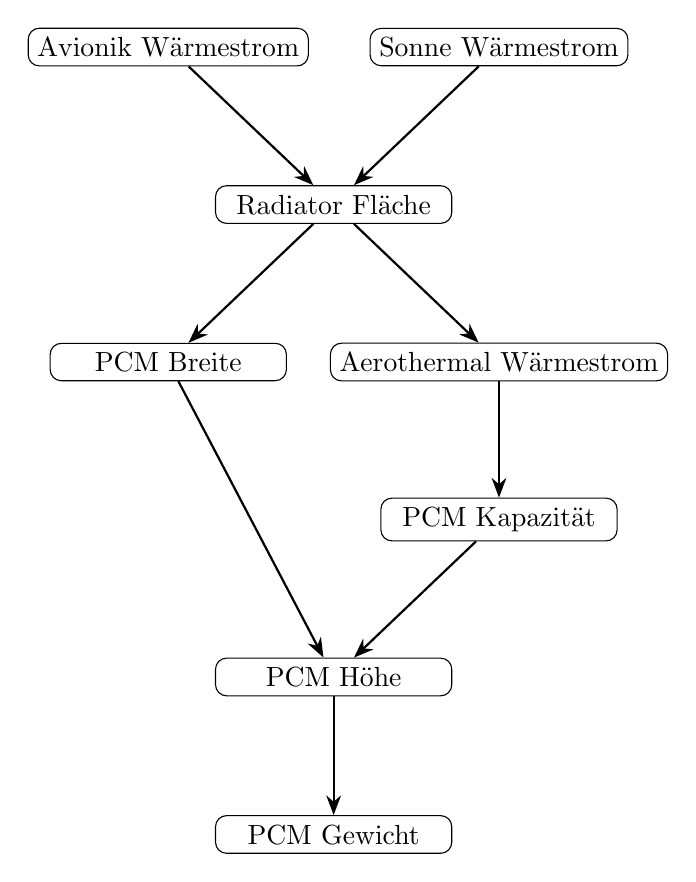
\begin{tikzpicture}[
    sibling distance=10em,
    every node/.style = {
      shape=rectangle,
      rounded corners,
      draw,
      align=center,
      minimum width=3cm
    },
    edge from parent/.style = {
      draw,
      ->,
      -{Stealth[length=0.25cm]},
      thick
    },
    arrow/.style = {
      ->,
      -{Stealth[length=0.25cm]},
      thick
    }
  ]

    % Top nodes
    \node (avionik) at (-2.1, 4) {Avionik Wärmestrom};
    \node (sonne)   at ( 2.1, 4) {Sonne Wärmestrom};

    % Radiator Fläche centered below
    \node (radiator) at (0, 2) {Radiator Fläche};

    % Children of Radiator
    \node (breite) at (-2.1, 0) {PCM Breite};
    \node (aerothermal) at (2.1, 0) {Aerothermal Wärmestrom};

    % PCM Kapazität as a separate node (not a child directly)
    \node (kapazitaet) at (2.1, -2) {PCM Kapazität};

    % PCM Höhe node below the center of breite and kapazitaet
    \node (hoehe) at (0, -4) {PCM Höhe};
    \node (gewicht) at (0, -6) {PCM Gewicht};

    % Arrows
    \draw[arrow] (avionik) -- (radiator);
    \draw[arrow] (sonne) -- (radiator);
    \draw[arrow] (radiator) -- (breite);
    \draw[arrow] (radiator) -- (aerothermal);
    \draw[arrow] (aerothermal) -- (kapazitaet);
    \draw[arrow] (breite) -- (hoehe);
    \draw[arrow] (kapazitaet) -- (hoehe);
    \draw[arrow] (hoehe) -- (gewicht);

  \end{tikzpicture}
  \caption{Dimensionierungs-Ablauf in der Vorauslegung}\label{fig:dimensionierung_ablauf}
\end{figure}
\newpage
\section{Thermales Interface}\label{thermalesInterface}
Hier gehts jetzt um wie die wärme verteilt und abtransportiert wird. Laut~\cite{Xingcun-2011} seite 35 geht die meiste Wärme in die PCB.
\newpage
\subsection{Thermal Straps}\label{thermalstraps}
Um das \ac{pcb} mit der Heatpipe zu verbinden werden Thermal Straps aus verschiedenen Materialien analysiert.
Thermal Straps sind flexible Verbindungsteile die Wärmebrücken zwischen mehreren Bauteilen gewehrleisten.
Wegen der hohe Wärmeleitzahl von \ac{pgs} und bedonders für Thermal Straps wichtigen Flexibilität, sind diese eine interessante Option.
Ein Nachteil von \ac{pgs} ist die geringe Dicke und der daraus resultierende geringe Querschnitt, welcher trotz hoher Wärmeleitzahl zu hoher Wärmestromdichte und stärkerer Temperaturerhöhung führen kann.
Im Vergleich mit herkömmlichen Materialien wie Aluminium und Kupfer soll ein Vergleich gezogen werden.
\begin{figure}[H]
  \centering
  \includegraphics[width=\textwidth]{thermal_straps_commercial.png}
  \caption{Kommerzeill erhältliche Thermal Straps aus Graphen, Kupfer und Aluminium der Firma Thermal Space and Thermal Straps}\label{fig:thermalstraps_commercial}
\end{figure}
\newpage
\section{CFD}\label{cfd}
\begin{figure}[H]
  \centering
  \includegraphics[width=\textwidth]{40WPCM_struktur.png}
  \caption{\ac{pcm} Struktur}\label{pcmstruktur}
\end{figure}
\begin{figure}
  \includegraphics[width=\textwidth]{40WPCM_mesh1.png}
  \caption{\ac{pcm} Mesh}\label{pcmmesh}
\end{figure}
%recoverytemperatur wahrscheinlich richtig noch recherchieren

% ----------- Diskussion & Schlussfolgerungen----------------------------------------
\newpage
\chapter{Ergebnisse}
\label{chap:Ergebnisse}
\begin{figure}[H]
  \centering
  \label{fig:pcm_waermestrom_flugsimulation}
  \includegraphics[width=\linewidth]{../../Code/pcm_radiator_hybrid_heatflux_during_flight.pdf}
  \caption{PCM Wärmestrom während Flug}
  \label{fig:re_pr_flugsimulation}
  \includegraphics[width=\linewidth]{../../Code/re_pr_during_flight.pdf}
  \caption{Reynolds- und Prandtlzahl während kritischer Phase im Flug}
\end{figure}

% ----------- Diskussion & Schlussfolgerungen----------------------------------------
\newpage
\chapter{Discussion and conclusions}
\label{chap:conclusion}

\section{Discussion about including pictures}


% ----------- Ausblick --------------------------------------------------------------
\newpage
\chapter{Zusammenfassung und Ausblick}
\label{chap:Ausblick}
\pagestyle{OnlySection}		% wie ganz oben definiert

Beispielliteraturverweise: 

\begin{enumerate}
	\item Fachzeitschrift
	\item Internetquelle
	\item Buch 
	\item Vorlesungsskript
\end{enumerate}

Anmerkung: Es gibt verschiedene Referenzierungsstile 


% ----------- Literatur -------------------------------------------------------------
\newpage
\renewcommand{\bibname}{Literaturverzeichnis}

\bibliography{Bibliography/quellen.bib}
\bibliographystyle{plain}%{unsrt}{abbrv}{abbrvnat}{unsrt}

\newpage

%----------- Anhang -----------------------------------------------------------------
\chapter*{Appendix}
\label{chapter:Appendix}
\pagestyle{Appendix}
\addcontentsline{toc}{chapter}{Appendix}

\section*{Appendix A: Simulationsergebnisse}\label{Anh:simulation}

\begin{figure}[H]
    \centering

    \begin{subfigure}{\textwidth}
        \centering
        \includegraphics[height=0.23\textheight]{ansyspost/airflow/maxQminus10-temperature-contour.png}
        \caption{maxQ -\SI{10}{\second}}
        \label{fig:maxQminus10_temp_contour}
    \end{subfigure}

    \begin{subfigure}{\textwidth}
        \centering
        \includegraphics[height=0.23\textheight]{ansyspost/airflow/maxQplus10-temperature-contour.png}
        \caption{maxQ +\SI{10}{\second}}
        \label{fig:maxQplus10_temp_contour}
    \end{subfigure}

    \begin{subfigure}{\textwidth}
        \centering
        \includegraphics[height=0.23\textheight]{ansyspost/airflow/maxQplus20-temperature-contour.png}
        \caption{maxQ +\SI{20}{\second}}
        \label{fig:maxQplus20_temp_contour}
    \end{subfigure}

    \caption{Statische Temperaturkontur der Luft}
    \label{fig:airflow_temp_contour_continued}
\end{figure}

\begin{figure}[H]
    \centering

    \begin{subfigure}{\textwidth}
        \centering
        \includegraphics[height=0.23\textheight]{ansyspost/airflow/maxQminus10-mach-contour.png}
        \caption{maxQ -\SI{10}{\second}}
        \label{fig:maxQminus10_mach_contour}
    \end{subfigure}

    \begin{subfigure}{\textwidth}
        \centering
        \includegraphics[height=0.23\textheight]{ansyspost/airflow/maxQplus10-mach-contour.png}
        \caption{maxQ +\SI{10}{\second}}
        \label{fig:maxQplus10_mach_contour}
    \end{subfigure}

    \begin{subfigure}{\textwidth}
        \centering
        \includegraphics[height=0.23\textheight]{ansyspost/airflow/maxQplus20-mach-contour.png}
        \caption{maxQ +\SI{20}{\second}}
        \label{fig:maxQplus20_mach_contour}
    \end{subfigure}

    \caption{Machzahlkontur der Luft}
    \label{fig:airflow_mach_contour_continued}
\end{figure}

\begin{figure}[H]
    \centering

    \begin{subfigure}[t]{0.14\textwidth}
        \centering
        \raisebox{1\height}{\includegraphics[height=0.2\textheight]{ansyspost/pcm/vector-legend.png}}
    \end{subfigure}%
    \hspace{2mm}% extra space between legend and first image
    \begin{subfigure}[t]{0.2\textwidth}
        \centering
        \includegraphics[height=0.7\textheight]{ansyspost/pcm/velocity-vector-300.png}
        \caption{\SI{300}{\second}}\label{fig:velocity_vector_300}
    \end{subfigure}%
    \begin{subfigure}[t]{0.2\textwidth}
        \centering
        \includegraphics[height=0.7\textheight]{ansyspost/pcm/velocity-vector-600.png}
        \caption{\SI{600}{\second}}\label{fig:velocity_vector_600}
    \end{subfigure}%
    \begin{subfigure}[t]{0.2\textwidth}
        \centering
        \includegraphics[height=0.7\textheight]{ansyspost/pcm/velocity-vector-900.png}
        \caption{\SI{900}{\second}}\label{fig:velocity_vector_900}
    \end{subfigure}%
    \begin{subfigure}[t]{0.2\textwidth}
        \centering
        \includegraphics[height=0.7\textheight]{ansyspost/pcm/velocity-vector-1200.png}
        \caption{\SI{1200}{\second}}\label{fig:velocity_vector_1200}
    \end{subfigure}
    \caption{Konturen der statischen Temperatur. Die Legende bezieht sich auf~\ref{fig:temperatur_1200}}\label{fig:pcm_static_temperature_kontur}
\end{figure}

\section*{Appendix B: bla}
\label{Anh:bla2}

%------------------------------------------------------------------------------------
\end{document}